\documentclass[12pt]{article}
\usepackage[margin=1in]{geometry}
\usepackage{amsmath, amssymb, amsthm, graphicx, hyperref}
\usepackage{amsmath}
\usepackage{enumerate}
\usepackage{fancyhdr}
\usepackage{multirow, multicol}
\usepackage{tikz}
\usepackage{wrapfig}
\pagestyle{fancy}
\usepackage{titlesec}
\usepackage{lastpage}
\usepackage{multirow}
\usepackage{indentfirst}
\fancyhead[LO]{JACK Z}
\fancyhead[RO]{Page \thepage\ of \pageref{LastPage}}
\usepackage{comment}
\newtheorem{definition}{Definition}
\usepackage{amsmath}
\usepackage{booktabs}
\usepackage{xcolor}
\usepackage{tcolorbox}  % For creating styled boxes
\tcbuselibrary{most}
\usepackage{tcolorbox} % for creating colored or framed text boxes
\tcbuselibrary{breakable} % allows tcolorboxes to break across pages

\definecolor{examplebg}{RGB}{255, 228, 225} % Light red background
\tcbuselibrary{theorems} 
\usepackage{graphicx}
\usepackage{booktabs} % For better table formatting
\usepackage{caption} % Essential for \captionof
\usepackage{tcolorbox} % For creating colored boxes
\tcbuselibrary{most} % Load most libraries for tcolorbox

\newtcbtheorem[number within=subsection]{Note}{Note}{
    colback=Black!5,
    colframe=white!35!black,
    fonttitle=\bfseries,
    colbacktitle=blue!85!black,
    coltitle=white,
    enhanced,
    attach boxed title to top left={yshift=-2mm, xshift=2mm},
    boxed title style={sharp corners},
    sharp corners
}{Not}

\newtcbtheorem[number within=subsection]{Definition}{Definition}{
    colback=blue!5,
    colframe=blue!35!black,
    fonttitle=\bfseries,
    colbacktitle=blue!85!black,
    coltitle=white,
    enhanced,
    attach boxed title to top left={yshift=-2mm, xshift=2mm},
    boxed title style={sharp corners},
    sharp corners
}{def}

\newtcbtheorem[number within=subsection]{mytheorem}{Theorem}{
    colback=orange!5,      % Background color of the box
    colframe=orange,     % Border color of the box
    coltitle=white,     % Color of theorem title
    colbacktitle=orange!85!black,, % Background color for the title
    fonttitle=\bfseries,
    title after break={Theorem \csname the\tcbcounter\endcsname\ -- Continued}, % for continued theorems
    enhanced,
    attach boxed title to top left={yshift=-2mm, xshift=2mm},
    boxed title style={sharp corners, colframe=black},
    sharp corners,
    separator sign none % no sign between title and theorem text
}{thm}


\usepackage{lipsum} % 生成示例文本
\usepackage{fancyhdr}

\pagestyle{fancy}
\fancyfoot[C]{%
  \begin{tcolorbox}[colback=blue!10, colframe=blue!35, boxrule=0.5pt, 
  sharp corners=south, boxsep=2pt, width=0.25\textwidth, 
  arc=3mm, enhanced, shadow=drop shadow]
    \centering
    {\textbf{\textcopyright\ \textit{Novel Prep}}}
  \end{tcolorbox}
}

% Define custom colors
\definecolor{deepblue}{rgb}{0.0, 0.18, 0.39}
\definecolor{deepred}{rgb}{0.6, 0, 0}

% Define theorem style
\newtheoremstyle{beautifulthm}
  {10pt} % Space above
  {10pt} % Space below
  {\itshape} % Body font
  {} % Indent amount
  {\bfseries\color{deepblue}} % Theorem head font
  {.} % Punctuation after theorem head
  {.5em} % Space after theorem head
  {} % Theorem head spec

\theoremstyle{beautifulthm}
\newtheorem{theorem}{Theorem}[section]

\begin{document}

\title{AP Calculus AB\&BC}
\author{Hongjun Zeng}
\maketitle
\lipsum[1-10] 

\tableofcontents
\begin{document}
\section{Limits and Continuity}
\section{Differentiation: Definition and Fundamental Properties}
\section{Differentiation: Composite, Implicit, and Inverse Function}
\section{Application of Differentiation}
\section{Analytical Applications of Differentiation}
\section{Accumulations of Change}
\section{Differential Equations}
\section{Applications of Integration}


\section{Parametric Equations, Polar Coordinates, and Vector-Valued Functions}

\newpage

\subsection{Defining and
Differentiating Parametric
Equations}


\subsubsection{Parametric Equations}

\begin{Definition}{Parametric Equations}{}
    
Parametric equations express $x$ and $y$ as functions of a third variable, called the parameter $t$, as follows:
\[
x = f(t), \quad y = g(t).
\]
Each value of $t$ corresponds to a point $(x, y)$, tracing out a parametric curve in the coordinate plane.


\begin{minipage}{\linewidth}
    \centering
    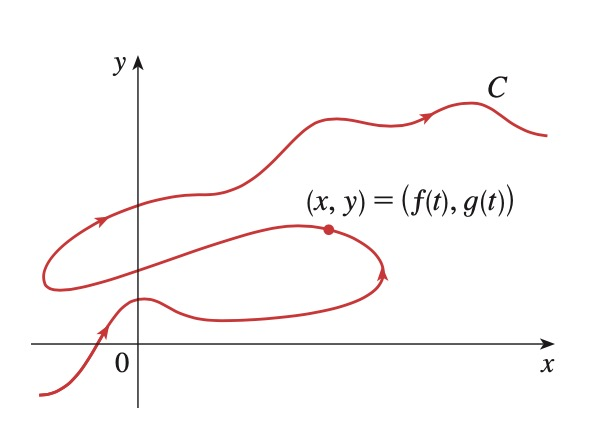
\includegraphics[width=0.50\linewidth]{Example_76.jpg} 
\end{minipage}
\end{Definition}

\begin{tcolorbox}[colback=examplebg, colframe=red!75!black, title=\textbf{EXAMPLE 2: Sketch and Identify the Parametric Curve}, fonttitle=\bfseries, sharp corners]

The parametric equations are given as:
\[
x = \cos t, \quad y = \sin t, \quad 0 \leq t \leq 2\pi
\]

\tcblower
\textbf{Solution:} 
If we plot the points $(x, y)$ as $t$ varies, it appears that the curve is a circle. To confirm this, we eliminate the parameter $t$. Observe that:
\[
x^2 + y^2 = \cos^2 t + \sin^2 t
\]
Using the Pythagorean identity:
\[
\cos^2 t + \sin^2 t = 1
\]
Thus, the equation becomes:
\[
x^2 + y^2 = 1
\]

This represents a circle with center at $(0, 0)$ and radius $1$.

\end{tcolorbox}






\begin{tcolorbox}[colback=examplebg, colframe=red!75!black, title=\textbf{EXAMPLE 1: Sketch and Identify the Parametric Curve}, fonttitle=\bfseries, sharp corners]

Sketch and identify the curve defined by the parametric equations:
\[
x = t^2 - 2t, \quad y = t + 1
\]



\tcblower
\textbf{Solution:} 

we sketch the curve by calculating $(x, y)$ for various values of $t$.

\textbf{Table of Points}
\[
\begin{array}{|c|c|c|}
\hline
t & x & y \\
\hline
-2 & 8 & -1 \\
-1 & 3 & 0 \\
0 & 0 & 1 \\
1 & -1 & 2 \\
2 & 0 & 3 \\
3 & 3 & 4 \\
4 & 8 & 5 \\
\hline
\end{array}
\]

\textbf{Graph of the Curve}

\begin{minipage}{\linewidth}
    \centering
    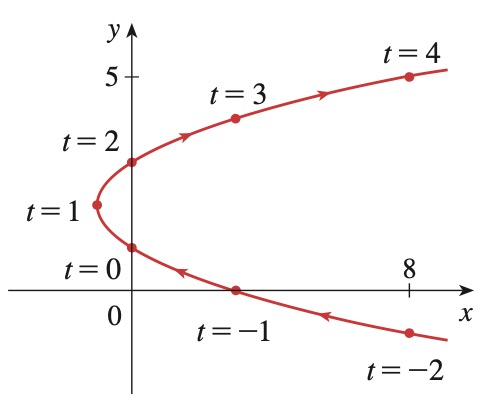
\includegraphics[width=0.40\linewidth]{Example_77.jpg} 
\end{minipage}
\end{tcolorbox}

\newpage
\subsubsection{Differentiating Parametric
Equations}

\begin{mytheorem}{Derivative of Parametric Equations}{}
Suppose $f$ and $g$ are differentiable functions of a parameter $t$, and the parametric curve is given by:
\[
x = f(t), \quad y = g(t).
\]
The slope of the tangent line to this curve is given by:
\[
\frac{dy}{dx} = \frac{\frac{dy}{dt}}{\frac{dx}{dt}},
\]
provided that $\frac{dx}{dt} \neq 0$. This result follows directly from the Chain Rule, as:
\[
\frac{dy}{dt} = \frac{dy}{dx} \cdot \frac{dx}{dt}.
\]


    
\end{mytheorem}



\begin{tcolorbox}[colback=examplebg, colframe=red!75!black, title=\textbf{EXAMPLE 1: Find the Integral of the Function}, fonttitle=\bfseries, sharp corners]
For the given parametric equations, eliminate the
parameter and write the corresponding
rectangular equation.
\textbf{Given:}
\begin{align*}
x &= e^{-t} \\
y &= e^{2t} - 1
\end{align*}

\tcblower
\textbf{Solution:} 
\begin{align*}
\ln x &= -t \quad \text{(taking the natural log of both sides)} \\
t &= -\ln x \\
y &= e^{2(-\ln x)} - 1 \\
y &= e^{\ln x^{-2}} - 1 \\
y &= x^{-2} - 1
\end{align*}

\textbf{Final Answer:} \( y = \frac{1}{x^2} - 1, \quad x > 0 \)
\end{tcolorbox}




\begin{tcolorbox}[colback=examplebg, colframe=red!75!black, title=\textbf{EXAMPLE 2: Tangent Line to the Parametric Curve}, fonttitle=\bfseries, sharp corners]
\textbf{Given:}
\begin{align*}
x &= t \cos t, \quad y = t \sin t
\end{align*}

\textbf{Find the tangent line at } t = \pi.


\tcblower
\textbf{Solution:} 
\textbf{Step 1: Compute the derivatives.}
\begin{align*}
\frac{dx}{dt} &= \cos t - t \sin t \\
\frac{dy}{dt} &= \sin t + t \cos t
\end{align*}

\textbf{Step 2: Find dy/dx} .
\begin{align*}
\frac{dy}{dx} &= \frac{\frac{dy}{dt}}{\frac{dx}{dt}} = \frac{\sin t + t \cos t}{\cos t - t \sin t}
\end{align*}

\textbf{Step 3: Evaluate at } t = \pi.
\begin{align*}
x(\pi) &= \pi \cos \pi = -\pi, \quad y(\pi) = \pi \sin \pi = 0 \\
\frac{dy}{dx}\Big|_{t = \pi} &= \frac{\sin \pi + \pi \cos \pi}{\cos \pi - \pi \sin \pi} = \frac{0 + \pi (-1)}{-1 - \pi (0)} = -\pi
\end{align*}

\textbf{Step 4: Write the tangent line.}
\begin{align*}
\text{Point: } (-\pi, 0), \quad \text{Slope: } -\pi \\
\text{Tangent line: } y &= -\pi (x + \pi)
\end{align*}

\textbf{Final Answer:} \( y = -\pi (x + \pi) \)
\end{tcolorbox}

\begin{tcolorbox}[colback=examplebg, colframe=red!75!black, title=\textbf{EXAMPLE 3: Determine the Tangent Line is Horizontal or Vertical}, fonttitle=\bfseries, sharp corners]
\textbf{Given:} A curve is defined parametrically by 
\[
x(t) = t^2, \quad y(t) = t^3 - 3t.
\]
Find the points on the graph where the tangent line is horizontal or vertical.


\tcblower
\textbf{Solution:} 
\textbf{Step 1: Compute dy/dx} .
\[
\frac{dx}{dt} = 2t, \quad \frac{dy}{dt} = 3t^2 - 3.
\]
\[
\frac{dy}{dx} = \frac{\frac{dy}{dt}}{\frac{dx}{dt}} = \frac{3t^2 - 3}{2t}.
\]

\textbf{Step 2: Find horizontal tangents.}

A tangent is horizontal when 
\[
\frac{dy}{dx} = 0 \implies 3t^2 - 3 = 0.
\]
\[
t^2 = 1 \implies t = \pm 1.
\]

For \( t = 1 \):
\[
x(1) = 1^2 = 1, \quad y(1) = 1^3 - 3(1) = -2.
\]
Point: \( (1, -2) \).

For \( t = -1 \):
\[
x(-1) = (-1)^2 = 1, \quad y(-1) = (-1)^3 - 3(-1) = 2.
\]
Point: \( (1, 2) \).

\textbf{Step 3: Find vertical tangents.}

A tangent is vertical when 
\[
\frac{dx}{dt} = 0 \implies 2t = 0.
\]
\[
t = 0.
\]

For \( t = 0 \):
\[
x(0) = 0^2 = 0, \quad y(0) = 0^3 - 3(0) = 0.
\]
Point: \( (0, 0) \).

\textbf{Final Answer:}
\[
\text{Horizontal tangents: } (1, -2) \text{ and } (1, 2).
\]
\[
\text{Vertical tangent: } (0, 0).
\]
\end{tcolorbox}




\newpage

\subsection{Second Derivatives of
Parametric Equations}

\noindent In previous topic, we knew the Derivative of Parametric Equations

\noindent Suppose $f$ and $g$ are differentiable functions of a parameter $t$, and the parametric curve is given by:
\[
x = f(t), \quad y = g(t).
\]
The slope of the tangent line to this curve is given by:
\[
\frac{dy}{dx} = \frac{\frac{dy}{dt}}{\frac{dx}{dt}},
\]
provided that $\frac{dx}{dt} \neq 0$. This result follows directly from the Chain Rule, as:
\[
\frac{dy}{dt} = \frac{dy}{dx} \cdot \frac{dx}{dt}.
\]



\begin{mytheorem}{Second Derivative of Parametric Equations}{}
   Let the parametric equations of a curve be given by 
\[
x = f(t), \quad y = g(t),
\]
where \(f\) and \(g\) are differentiable functions of \(t\), and \(\frac{dx}{dt} \neq 0\). Then, the second derivative of \(y\) with respect to \(x\) is given by
\[
\frac{d^2y}{dx^2} = \frac{\frac{d}{dt}\left(\frac{dy}{dx}\right)}{\frac{dx}{dt}},
\]
where \(\frac{dy}{dx}\) is the first derivative of \(y\) with respect to \(x\), expressed as
\[
\frac{dy}{dx} = \frac{\frac{dy}{dt}}{\frac{dx}{dt}}.
\] 
\end{mytheorem}


\begin{tcolorbox}[colback=examplebg, colframe=red!75!black, title=\textbf{EXAMPLE 1: Find the Derivetive of the Parametric Equation}, fonttitle=\bfseries, sharp corners]
Given the parametric equations 
\[
x = 3t^2 - 1 \quad \text{and} \quad y = \ln t,
\]
find \(\frac{d^2y}{dx^2}\) in terms of \(t\).


\tcblower
\textbf{Solution:} 
First, compute \(\frac{dy}{dx}\):
\[
\frac{dy}{dx} = \frac{\frac{dy}{dt}}{\frac{dx}{dt}} = \frac{\frac{1}{t}}{6t} = \frac{1}{6t^2}.
\]

Next, compute \(\frac{d^2y}{dx^2}\) using the formula:
\[
\frac{d^2y}{dx^2} = \frac{\frac{d}{dt}\left(\frac{dy}{dx}\right)}{\frac{dx}{dt}}.
\]
Since \(\frac{dy}{dx} = \frac{1}{6t^2}\), differentiate with respect to \(t\):
\[
\frac{d}{dt}\left(\frac{1}{6t^2}\right) = -\frac{1}{3t^3}.
\]

Now divide by \(\frac{dx}{dt} = 6t\):
\[
\frac{d^2y}{dx^2} = \frac{-\frac{1}{3t^3}}{6t} = -\frac{1}{3t^3} \cdot \frac{1}{6t} = -\frac{1}{18t^4}.
\]

Thus, the second derivative is:
\[
\frac{d^2y}{dx^2} = -\frac{1}{18t^4}.
\]
\end{tcolorbox}

\begin{tcolorbox}[colback=examplebg, colframe=red!75!black, title=\textbf{EXAMPLE 2: Concavity}, fonttitle=\bfseries, sharp corners]
Given the parametric equations \( x = \theta - \cos \theta \) and \( y = 1 - \sin \theta \), find the slope and concavity at \( \theta = \pi \).



\tcblower
\textbf{Solution:} 
\textbf{Slope:}
\[
\frac{dy}{dx} = \frac{\frac{dy}{d\theta}}{\frac{dx}{d\theta}} = \frac{-\cos \theta}{1 + \sin \theta}.
\]
At \( \theta = \pi \):
\[
\frac{dy}{dx} = \frac{-\cos \pi}{1 + \sin \pi} = \frac{-(-1)}{1 + 0} = 1.
\]

\textbf{Concavity:}
\[
\frac{d^2y}{dx^2} = \frac{\frac{d}{d\theta}\left(\frac{dy}{dx}\right)}{\frac{dx}{d\theta}} = \frac{\sin \theta (1 + \sin \theta) - (-\cos \theta)(\cos \theta)}{(1 + \sin \theta)^2} \cdot \frac{1}{1 + \sin \theta}.
\]
Simplify the numerator:
\[
\sin \theta (1 + \sin \theta) - (-\cos \theta)(\cos \theta) = \sin \theta (1 + \sin \theta) + \cos^2 \theta.
\]
At \( \theta = \pi \):
\[
\sin \pi (1 + \sin \pi) + \cos^2 \pi = 0 \cdot (1 + 0) + (-1)^2 = 1.
\]
Thus:
\[
\frac{d^2y}{dx^2} = \frac{1}{1} = 1 \quad \text{(Concave up)}.
\]
\end{tcolorbox}







\begin{tcolorbox}[colback=examplebg, colframe=red!75!black, title=\textbf{EXAMPLE 3: Practice of Parametric Equations}, fonttitle=\bfseries, sharp corners]
A curve \( C \) is defined by the parametric equations \( x = t^2 \), \( y = t^3 - 3t \):
\begin{enumerate}
    \item[(a)] Show that \( C \) has two tangents at the point \( (3, 0) \) and find their equations.
    \item[(b)] Find the points on \( C \) where the tangent is horizontal or vertical.
    \item[(c)] Determine where the curve is concave upward or downward.
\end{enumerate}


\tcblower
\textbf{Solution:} 
\begin{enumerate}
    \item[(a)] Notice that \( x = 3 \) for \( t = \pm \sqrt{3} \), and in both cases, \( y = t(t^2 - 3) = 0 \). Therefore, the point \( (3, 0) \) on \( C \) arises from two values of the parameter, \( t = \sqrt{3} \) and \( t = -\sqrt{3} \). This indicates that \( C \) crosses itself at \( (3, 0) \).

    Since
    \[
    \frac{dy}{dx} = \frac{\frac{dy}{dt}}{\frac{dx}{dt}} = \frac{3t^2 - 3}{2t},
    \]
    the slope of the tangent when \( t = \sqrt{3} \) is
    \[
    \frac{dy}{dx} = \frac{6}{2\sqrt{3}} = \sqrt{3},
    \]
    and when \( t = -\sqrt{3} \), the slope is
    \[
    \frac{dy}{dx} = \frac{-6}{2\sqrt{3}} = -\sqrt{3}.
    \]
    Thus, we have two different tangent lines at \( (3, 0) \) with equations:
    \[
    y = \sqrt{3}(x - 3) \quad \text{and} \quad y = -\sqrt{3}(x - 3).
    \]

    \item[(b)] \( C \) has a horizontal tangent when \( \frac{dy}{dx} = 0 \), that is, when \( \frac{dy}{dt} = 0 \) and \( \frac{dx}{dt} \neq 0 \). Since \( \frac{dy}{dt} = 3t^2 - 3 \), this happens when \( t^2 = 1 \), that is, \( t = \pm 1 \). The corresponding points on \( C \) are \( (1, -2) \) and \( (1, 2) \).

    \( C \) has a vertical tangent when \( \frac{dx}{dt} = 2t = 0 \), that is, \( t = 0 \). The corresponding point on \( C \) is \( (0, 0) \).

    \item[(c)] The concavity of the curve is determined by the sign of \( \frac{d^2y}{dx^2} \):
    \[
    \frac{d^2y}{dx^2} = \frac{\frac{d}{dt}\left(\frac{dy}{dx}\right)}{\frac{dx}{dt}}.
    \]
    Compute \( \frac{d}{dt}\left(\frac{dy}{dx}\right) \) and determine the intervals where \( \frac{d^2y}{dx^2} > 0 \) (concave up) or \( \frac{d^2y}{dx^2} < 0 \) (concave down).
\end{enumerate}
\end{tcolorbox}


\subsection{Finding Arc Lengths
of Curves Given by
Parametric Equations}

\subsubsection{Arc Length of a Curve}
\begin{Definition}{Arc Lengths}{}
    The arc length of a smooth curve \( y = f(x) \), defined over the interval \([a, b]\). It refers to the distance between two points on a curve.

\begin{minipage}{\linewidth}
    \centering
    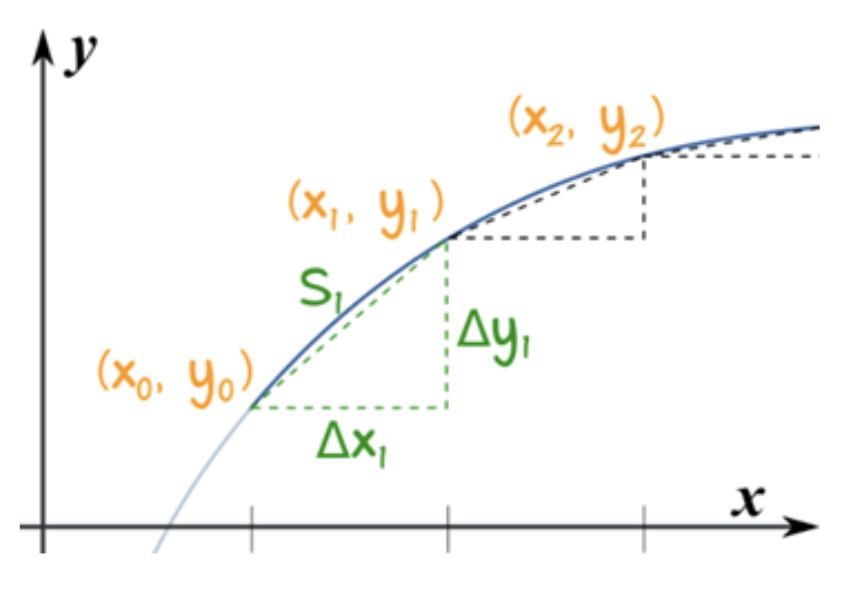
\includegraphics[width=0.40\linewidth]{Example_78.jpg} 
\end{minipage}

\end{Definition}


\begin{mytheorem}{Arc Length Formula}{}
    If \( f'(x) \) is continuous on the interval \([a, b]\), then the length of the curve \( y = f(x) \) from \( x = a \) to \( x = b \) is given by:
\[
L = \int_a^b \sqrt{1 + [f'(x)]^2} \, dx.
\]

Using Leibniz notation for derivatives, the arc length formula can also be expressed as:
\[
L = \int_a^b \sqrt{1 + \left( \frac{dy}{dx} \right)^2} \, dx.
\]
\end{mytheorem}

\begin{tcolorbox}[colback=examplebg, colframe=red!75!black, title=\textbf{EXAMPLE 1: Find the Arc Length of the Function}, fonttitle=\bfseries, sharp corners]

Find the length of the arc of the semicubical parabola \( y^2 = x^3 \) between the points \( (1, 1) \) and \( (4, 8) \).

\tcblower
\textbf{Solution:} 
For the top half of the curve, we have:
\[
y = x^{3/2}, \quad \frac{dy}{dx} = \frac{3}{2}x^{1/2}.
\]

Using the arc length formula:
\[
L = \int_1^4 \sqrt{1 + \left( \frac{3}{2}x^{1/2} \right)^2} \, dx = \int_1^4 \sqrt{1 + \frac{9}{4}x} \, dx.
\]
\end{tcolorbox}


\subsubsection{Arc Length of Parametric Curves}
\begin{mytheorem}{Arc Length of Parametric Curves}{}
    If a curve \( C \) is described by the parametric equations \( x = f(t) \), \( y = g(t) \), \( \alpha \leq t \leq \beta \), where \( f'(t) \) and \( g'(t) \) are continuous on \([ \alpha, \beta ]\) and \( C \) is traversed exactly once as \( t \) increases from \( \alpha \) to \( \beta \), then the length of \( C \) is given by:
\[
L = \int_\alpha^\beta \sqrt{\left( \frac{dx}{dt} \right)^2 + \left( \frac{dy}{dt} \right)^2} \, dt.
\]
\end{mytheorem}


\begin{tcolorbox}[colback=examplebg, colframe=red!75!black, title=\textbf{EXAMPLE 1: Arc Length of Parametric Equation}, fonttitle=\bfseries, sharp corners]

For the paramatric equation
\[
x = \cos t, \quad y = \sin t, \quad 0 \leq t \leq 2\pi,
\]
Find the Arc length of the parametric equation 


\tcblower
\textbf{Solution:} 

\[
\frac{dx}{dt} = -\sin t, \quad \frac{dy}{dt} = \cos t.
\]
Using Theorem , the arc length $L$ is:
\[
L = \int_0^{2\pi} \sqrt{\left(\frac{dx}{dt}\right)^2 + \left(\frac{dy}{dt}\right)^2} \, dt = \int_0^{2\pi} \sqrt{\sin^2 t + \cos^2 t} \, dt = \int_0^{2\pi} 1 \, dt = 2\pi.
\]
\end{tcolorbox}



\begin{tcolorbox}[colback=examplebg, colframe=red!75!black, title=\textbf{EXAMPLE 2: Arc Length of Parametric Equation}, fonttitle=\bfseries, sharp corners]

The position of a particle at time $t$ is given by the parametric equations:
\[
x = 2t + 3, \quad y = 4t^2, \quad t \geq 0.
\]
Find the speed of the particle when it is at the point $(5, 4)$.

\tcblower
\textbf{Solution:} 
 the speed of the particle at any time $t$ is:
\[
v(t) = \sqrt{\left(\frac{dx}{dt}\right)^2 + \left(\frac{dy}{dt}\right)^2} = \sqrt{2^2 + (8t)^2} = 2\sqrt{1 + 16t^2}.
\]

The particle is at the point $(5, 4)$ when $t = 1$, so its speed at that point is:
\[
v(1) = 2\sqrt{1 + 16(1)^2} = 2\sqrt{17} \approx 8.25.
\]

\end{tcolorbox}


\newpage

\subsection{Defining and Differentiating Vector-Valued Functions}
\subsubsection{Vector}

\begin{Definition}{Vector}{}
A \textit{vector} is a quantity that has both \textbf{magnitude} (size or length) and \textbf{direction}. It is often used to represent physical quantities like velocity, force, or displacement. 

Vectors are typically written in the form:
\[
\vec{v} = \langle v_1, v_2, \dots, v_n \rangle,
\]
where $v_1, v_2, \dots, v_n$ are the components of the vector in an $n$-dimensional space.
\end{Definition}
\textbf{Key Features}


\begin{enumerate}
    \item \textbf{Magnitude (Length):} The magnitude of a vector $\vec{v} = \langle v_1, v_2 \rangle$ in 2D is:
    \[
    \|\vec{v}\| = \sqrt{v_1^2 + v_2^2}.
    \]
    For an $n$-dimensional vector $\vec{v} = \langle v_1, v_2, \dots, v_n \rangle$:
    \[
    \|\vec{v}\| = \sqrt{v_1^2 + v_2^2 + \cdots + v_n^2}.
    \]

    \item \textbf{Direction:} The direction of a vector is given by the orientation of its components relative to the coordinate axes.

\end{enumerate}

\begin{tcolorbox}[colback=examplebg, colframe=red!75!black, title=\textbf{EXAMPLE 1: Find the Magnitude and Direction of the Vector}, fonttitle=\bfseries, sharp corners]

Consider the vector $\vec{v} = \langle 6, 8 \rangle$:
\begin{itemize}
    \item \textbf{Magnitude:}
    \[
    \|\vec{v}\| = \sqrt{6^2 + 8^2} = \sqrt{36 + 64} = 10.
    \]
    \item \textbf{Direction:} The vector points from the origin $(0, 0)$ to the point $(6, 8)$.
\end{itemize}


\begin{minipage}{\linewidth}
    \centering
    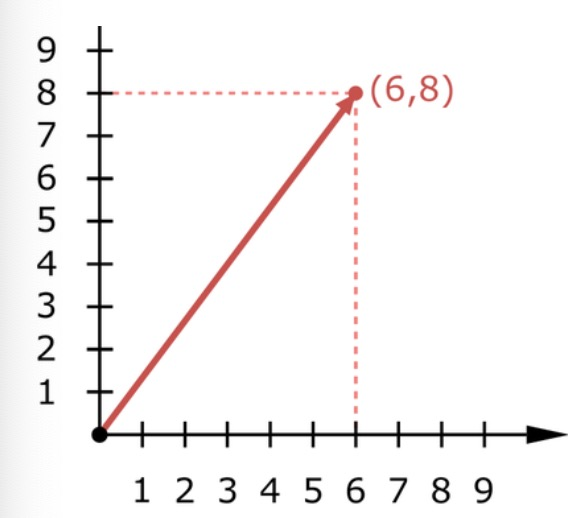
\includegraphics[width=0.40\linewidth]{Example_79.jpg} 
\end{minipage}

\end{tcolorbox}



\subsubsection{Vector-Valued Functions}

\begin{Definition}{Vector-Valued Function}{}
    A function of the form
\[
\vec{r}(t) = f(t)\mathbf{i} + g(t)\mathbf{j} \quad \text{(Plane)}
\]
or
\[
\vec{r}(t) = f(t)\mathbf{i} + g(t)\mathbf{j} + h(t)\mathbf{k} \quad \text{(Space)}
\]
is called a \textbf{vector-valued function}, where the \textbf{component functions} $f$, $g$, and $h$ are real-valued functions of the parameter $t$.

Vector-valued functions can also be expressed using angle brackets:
\[
\vec{r}(t) = \langle f(t), g(t) \rangle \quad \text{(Plane)},
\]
or
\[
\vec{r}(t) = \langle f(t), g(t), h(t) \rangle \quad \text{(Space)}.
\]
\end{Definition}


\begin{mytheorem}{Differentiation of Vector-Valued Functions}{}



1. If $\vec{r}(t) = f(t)\mathbf{i} + g(t)\mathbf{j}$, where $f$ and $g$ are differentiable functions of $t$, then:
\[
\vec{r}'(t) = f'(t)\mathbf{i} + g'(t)\mathbf{j} \quad \text{(Plane)}.
\]

2. If $\vec{r}(t) = f(t)\mathbf{i} + g(t)\mathbf{j} + h(t)\mathbf{k}$, where $f$, $g$, and $h$ are differentiable functions of $t$, then:
\[
\vec{r}'(t) = f'(t)\mathbf{i} + g'(t)\mathbf{j} + h'(t)\mathbf{k} \quad \text{(Space)}.
\]
    
\end{mytheorem}


\begin{tcolorbox}[colback=examplebg, colframe=red!75!black, title=\textbf{EXAMPLE 2: Finding the Derivative of a Vector-Valued Function}, fonttitle=\bfseries, sharp corners]
Given the vector-valued function:
\[
\vec{r}(t) = \langle 4t^2, 7t^7 \rangle,
\]
find $\vec{r}'(4)$.


\tcblower
\textbf{Solution:} 

To find $\vec{r}'(t)$, differentiate each component of $\vec{r}(t)$ with respect to $t$:
\begin{itemize}
    \item The horizontal component $4t^2$ differentiates to $8t$.
    \item The vertical component $7t^7$ differentiates to $49t^6$.
\end{itemize}
\[
\vec{r}'(4) = \langle 32, 49 \cdot 4096 \rangle = \langle 32, 200704 \rangle.
\]
\end{tcolorbox}


\begin{tcolorbox}[colback=examplebg, colframe=red!75!black, title=\textbf{EXAMPLE 3: Differentiation of a Vector-Valued Function}, fonttitle=\bfseries, sharp corners]

For the vector-valued function:
\[
\vec{r}(t) = t\mathbf{i} + (t^2 + 2)\mathbf{j},
\]
find $\vec{r}'(t)$. Then, sketch the plane curve represented by $\vec{r}(t)$ and the graphs of $\vec{r}(1)$ and $\vec{r}'(1)$.

\tcblower
\textbf{Solution:} 
Differentiate on a component-by-component basis to obtain:
\[
\vec{r}'(t) = \mathbf{i} + 2t\mathbf{j}.
\]

From the position vector $\vec{r}(t)$, you can write the parametric equations:
\[
x = t \quad \text{and} \quad y = t^2 + 2.
\]
The corresponding rectangular equation is:
\[
y = x^2 + 2.
\]

When $t = 1$:
\[
\vec{r}(1) = \mathbf{i} + 3\mathbf{j},
\]
and:
\[
\vec{r}'(1) = \mathbf{i} + 2\mathbf{j}.
\]
\end{tcolorbox}


\begin{mytheorem}{Properties of the Derivative}{}

    
Let $\vec{r}$ and $\vec{u}$ be differentiable vector-valued functions of $t$, let $w$ be a differentiable real-valued function of $t$, and let $c$ be a scalar. The following properties hold:

\begin{enumerate}
    \item \textbf{Scalar Multiplication:}
    \[
    \frac{d}{dt} \left[ c \vec{r}(t) \right] = c \vec{r}'(t)
    \]

    \item \textbf{Addition and Subtraction:}
    \[
    \frac{d}{dt} \left[ \vec{r}(t) \pm \vec{u}(t) \right] = \vec{r}'(t) \pm \vec{u}'(t)
    \]

    \item \textbf{Scalar-Vector Multiplication:}
    \[
    \frac{d}{dt} \left[ w(t) \vec{r}(t) \right] = w(t) \vec{r}'(t) + w'(t) \vec{r}(t)
    \]

    \item \textbf{Dot Product:}
    \[
    \frac{d}{dt} \left[ \vec{r}(t) \cdot \vec{u}(t) \right] = \vec{r}(t) \cdot \vec{u}'(t) + \vec{r}'(t) \cdot \vec{u}(t)
    \]

    \item \textbf{Composition:}
    \[
    \frac{d}{dt} \left[ \vec{r}(w(t)) \right] = \vec{r}'(w(t)) w'(t)
    \]

    \item \textbf{Orthogonality:}
    If $\vec{r}(t) \cdot \vec{r}(t) = c$ (a constant), then:
    \[
    \vec{r}(t) \cdot \vec{r}'(t) = 0.
    \]
\end{enumerate}
\end{mytheorem}


\begin{tcolorbox}[colback=examplebg, colframe=red!75!black, title=\textbf{EXAMPLE 4: Using Properties of the Derivative}, fonttitle=\bfseries, sharp corners]

For $\vec{r}(t) = \frac{1}{t} \vec{i} - \vec{j} + \ln t \, \vec{k}$ and $\vec{u}(t) = t^2 \vec{i} - 2t \vec{j} + \vec{k}$, find:

\[
\frac{d}{dt} \left[ \vec{r}(t) \cdot \vec{u}(t) \right].
\]

\tcblower
\textbf{Solution:} 
Using the product rule for the dot product:
\[
\frac{d}{dt} \left[ \vec{r}(t) \cdot \vec{u}(t) \right] = \vec{r}'(t) \cdot \vec{u}(t) + \vec{r}(t) \cdot \vec{u}'(t).
\]

First, compute the derivatives:
\[
\vec{r}'(t) = -\frac{1}{t^2} \vec{i} + \frac{1}{t} \vec{k}, \quad \vec{u}'(t) = 2t \vec{i} - 2 \vec{j}.
\]

Substitute into the formula:
\[
\frac{d}{dt} \left[ \vec{r}(t) \cdot \vec{u}(t) \right] = \vec{r}'(t) \cdot \vec{u}(t) + \vec{r}(t) \cdot \vec{u}'(t).
\]

Expand each term:

1. Compute $\vec{r}'(t) \cdot \vec{u}(t)$:
\[
\vec{r}'(t) \cdot \vec{u}(t) = \left(-\frac{1}{t^2} \vec{i} + \frac{1}{t} \vec{k} \right) \cdot \left( t^2 \vec{i} - 2t \vec{j} + \vec{k} \right),
\]
\[
= -\frac{1}{t^2} (t^2) + \frac{1}{t} (1) = -1 + \frac{1}{t}.
\]

2. Compute $\vec{r}(t) \cdot \vec{u}'(t)$:
\[
\vec{r}(t) \cdot \vec{u}'(t) = \left( \frac{1}{t} \vec{i} - \vec{j} + \ln t \, \vec{k} \right) \cdot \left( 2t \vec{i} - 2 \vec{j} \right),
\]
\[
= \frac{1}{t} (2t) + (-1)(-2) + (\ln t)(0) = 2 + 2 = 4.
\]

Combine the results:
\[
\frac{d}{dt} \left[ \vec{r}(t) \cdot \vec{u}(t) \right] = (-1 + \frac{1}{t}) + 4 = 3 + \frac{1}{t}.
\]
\end{tcolorbox}


\newpage
\subsection{Integrating Vector-Valued Functions}

\begin{Definition}{Integration of Vector-Valued Functions}{}
    


\textbf{1. Plane (Two-Dimensional Space)}
If $\vec{r}(t) = f(t) \vec{i} + g(t) \vec{j}$, where $f$ and $g$ are continuous on $[a, b]$, then:
\begin{itemize}
    \item The \textbf{indefinite integral (antiderivative)} of $\vec{r}$ is:
    \[
    \int \vec{r}(t) \, dt = \left[ \int f(t) \, dt \right] \vec{i} + \left[ \int g(t) \, dt \right] \vec{j}.
    \]
    \item The \textbf{definite integral} over the interval $a \leq t \leq b$ is:
    \[
    \int_a^b \vec{r}(t) \, dt = \left[ \int_a^b f(t) \, dt \right] \vec{i} + \left[ \int_a^b g(t) \, dt \right] \vec{j}.
    \]
\end{itemize}

\textbf{2. Space (Three-Dimensional Space)}
If $\vec{r}(t) = f(t) \vec{i} + g(t) \vec{j} + h(t) \vec{k}$, where $f$, $g$, and $h$ are continuous on $[a, b]$, then:
\begin{itemize}
    \item The \textbf{indefinite integral (antiderivative)} of $\vec{r}$ is:
    \[
    \int \vec{r}(t) \, dt = \left[ \int f(t) \, dt \right] \vec{i} + \left[ \int g(t) \, dt \right] \vec{j} + \left[ \int h(t) \, dt \right] \vec{k}.
    \]
    \item The \textbf{definite integral} over the interval $a \leq t \leq b$ is:
    \[
    \int_a^b \vec{r}(t) \, dt = \left[ \int_a^b f(t) \, dt \right] \vec{i} + \left[ \int_a^b g(t) \, dt \right] \vec{j} + \left[ \int_a^b h(t) \, dt \right] \vec{k}.
    \]
\end{itemize}

\end{Definition}

\begin{tcolorbox}[colback=examplebg, colframe=red!75!black, title=\textbf{EXAMPLE 1: Definite Integral of a Vector-Valued Function}, fonttitle=\bfseries, sharp corners]


Evaluate the integral:
\[
\int_{0}^{1} \vec{r}(t) \, dt = \int_{0}^{1} \left( 3\sqrt{t} \, \vec{i} + \frac{1}{t+1} \, \vec{j} + e^{-t} \, \vec{k} \right) dt.
\]
\tcblower
\textbf{Solution:} 

Breaking the integral into components:
\[
\int_{0}^{1} \vec{r}(t) \, dt = \left( \int_{0}^{1} 3t^{1/2} \, dt \right) \vec{i} + \left( \int_{0}^{1} \frac{1}{t+1} \, dt \right) \vec{j} + \left( \int_{0}^{1} e^{-t} \, dt \right) \vec{k}.
\]

Evaluating each integral:
\[
\int_{0}^{1} 3t^{1/2} \, dt = \left[ 2t^{3/2} \right]_{0}^{1} = 2(1)^{3/2} - 2(0)^{3/2} = 2,
\]
\[
\int_{0}^{1} \frac{1}{t+1} \, dt = \ln|t+1| \Big|_{0}^{1} = \ln(2) - \ln(1) = \ln(2),
\]
\[
\int_{0}^{1} e^{-t} \, dt = \left[ -e^{-t} \right]_{0}^{1} = -(e^{-1} - e^{0}) = 1 - \frac{1}{e}.
\]

Substituting back:
\[
\int_{0}^{1} \vec{r}(t) \, dt = \left( 2 \right) \vec{i} + \left( \ln(2) \right) \vec{j} + \left( 1 - \frac{1}{e} \right) \vec{k}.
\]
\end{tcolorbox}


\begin{tcolorbox}[colback=examplebg, colframe=red!75!black, title=\textbf{EXAMPLE 2: Integrating a Vector-Valued Function}, fonttitle=\bfseries, sharp corners]

Find the indefinite integral:
\[
\int \left( t \vec{i} + 3 \vec{j} \right) \, dt.
\]

\tcblower
\textbf{Solution:} 
Integrate component-wise:
\[
\int \left( t \vec{i} + 3 \vec{j} \right) \, dt = \left( \int t \, dt \right) \vec{i} + \left( \int 3 \, dt \right) \vec{j}.
\]

Evaluating the integrals:
\[
\int t \, dt = \frac{t^2}{2}, \quad \int 3 \, dt = 3t.
\]

Including the constant of integration:
\[
\int \left( t \vec{i} + 3 \vec{j} \right) \, dt = \frac{t^2}{2} \vec{i} + 3t \vec{j} + \vec{C}.
\]

\end{tcolorbox}


\begin{tcolorbox}[colback=examplebg, colframe=red!75!black, title=\textbf{EXAMPLE 3: The Antiderivative of a Vector-Valued Function}, fonttitle=\bfseries, sharp corners]

Find the antiderivative of:
\[
\vec{r}'(t) = \cos(2t) \vec{i} - 2\sin(t) \vec{j} + \frac{1}{1+t^2} \vec{k},
\]
such that:
\[
\vec{r}(0) = 3 \vec{i} - 2 \vec{j} + \vec{k}.
\]

\tcblower
\textbf{Solution:} 
Integrating component-wise:
\[
\vec{r}(t) = \int \cos(2t) \, dt \, \vec{i} + \int -2\sin(t) \, dt \, \vec{j} + \int \frac{1}{1+t^2} \, dt \, \vec{k}.
\]



Assembling the vector:
\[
\vec{r}(t) = \left( \frac{1}{2}\sin(2t) + C_1 \right) \vec{i} + \left( 2\cos(t) + C_2 \right) \vec{j} + \left( \arctan(t) + C_3 \right) \vec{k}.
\]

Using the initial condition $\vec{r}(0) = 3 \vec{i} - 2 \vec{j} + \vec{k}$:
\[
\vec{r}(0) = \left( \frac{1}{2}\sin(0) + C_1 \right) \vec{i} + \left( 2\cos(0) + C_2 \right) \vec{j} + \left( \arctan(0) + C_3 \right) \vec{k}.
\]

This simplifies to:
\[
C_1 = 3, \quad C_2 = -4, \quad C_3 = 1.
\]
\end{tcolorbox}

\subsection{Solving Motion Problems
Using Parametric and
Vector-Valued Functions}

\subsubsection{Motion Terms}
\begin{Note}{Motion Terms}{}
    \begin{enumerate}
    \item **Position** ($\vec{r}(t)$):\\
    The location of an object in space at a specific time $t$. It is often represented as a vector:
    \[
    \vec{r}(t) = \langle x(t), y(t), z(t) \rangle.
    \]

    \item **Displacement** ($\Delta \vec{r}$):\\
    The change in position of an object from one point to another. It is given by:
    \[
    \Delta \vec{r} = \vec{r}(t_2) - \vec{r}(t_1).
    \]
    Displacement is a vector quantity with both magnitude and direction.

    \item **Distance**:\\
    The total length of the path traveled by an object, irrespective of direction. Unlike displacement, distance is a scalar quantity.

    \item **Velocity** ($\vec{v}(t)$):\\
    The rate of change of position with respect to time. It is the derivative of the position vector:
    \[
    \vec{v}(t) = \frac{d\vec{r}(t)}{dt}.
    \]
    Velocity is a vector and describes both the speed and direction of motion.

    \item **Acceleration** ($\vec{a}(t)$):\\
    The rate of change of velocity with respect to time. It is the derivative of the velocity vector:
    \[
    \vec{a}(t) = \frac{d\vec{v}(t)}{dt}.
    \]
    Acceleration is also a vector and indicates how the velocity changes over time.
\end{enumerate}
\end{Note}

\begin{minipage}{\linewidth}
    \centering
    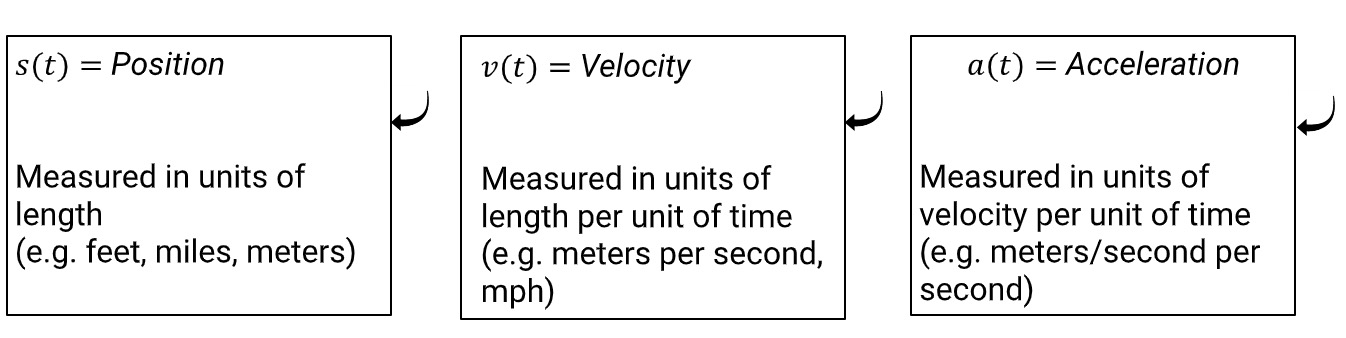
\includegraphics[width=1.0\linewidth]{Example_17.jpg} % Adjust the image width as necessary
    \captionof{figure}{}
    \label{fig:graph}
\end{minipage}

\newpage
\subsubsection{Calculus with Vector-Valued Functions}

\begin{mytheorem}{Velocity and Acceleration in Vector-Valued Functions}{}

If $x$ and $y$ are twice-differentiable functions of $t$, and $\vec{r}$ is a vector-valued function given by:
\[
\vec{r}(t) = x(t)\vec{i} + y(t)\vec{j},
\]
then the following definitions apply:

\begin{enumerate}
    \item **Velocity** ($\vec{v}(t)$):\\
    The velocity vector is the first derivative of the position vector $\vec{r}(t)$ with respect to time $t$:
    \[
    \vec{v}(t) = \vec{r}'(t) = x'(t)\vec{i} + y'(t)\vec{j}.
    \]

    \item **Acceleration** ($\vec{a}(t)$):\\
    The acceleration vector is the first derivative of the velocity vector $\vec{v}(t)$ or the second derivative of the position vector $\vec{r}(t)$ with respect to time $t$:
    \[
    \vec{a}(t) = \vec{r}''(t) = x''(t)\vec{i} + y''(t)\vec{j}.
    \]

    \item **Speed** ($\|\vec{v}(t)\|$):\\
    The speed is the magnitude (norm) of the velocity vector:
    \[
    \|\vec{v}(t)\| = \|\vec{r}'(t)\| = \sqrt{\big[x'(t)\big]^2 + \big[y'(t)\big]^2}.
    \]
\end{enumerate}
    
\end{mytheorem}

\begin{mytheorem}{Displacement in Vector-Valued Functions}{}
    
\begin{enumerate}
    \begin{itemize}

        \item The displacement vector $\Delta \vec{r}$ can be found by integrating the velocity vector $\vec{v}(t)$ over a given time interval $[a, b]$:

\[
\Delta \vec{r} = \int_a^b \vec{v}(t) \, dt.
\]
    \end{itemize}
\end{enumerate}

\end{mytheorem}

\begin{mytheorem}{Distance}{}
 \begin{enumerate}
        Distance represents the total length of the path traveled by the object and is calculated using the arc length formula for vector-valued functions:
        \[
        \text{Distance} = \int_a^b \|\vec{v}(t)\| \, dt,
        \]
\end{enumerate}
\end{mytheorem}


\begin{tcolorbox}[colback=examplebg, colframe=red!75!black, title=\textbf{EXAMPLE 1: Finding the Displacement Vector}, fonttitle=\bfseries, sharp corners]
Given a velocity vector $\vec{v}(t) = \langle 3t^2, 2t \rangle$, find the displacement vector $\Delta \vec{r}$ over the interval $[2, 5]$.


\tcblower
\textbf{Solution:} 
The displacement vector $\Delta \vec{r}$ is given by:
\[
\Delta \vec{r} = \langle \Delta x, \Delta y \rangle,
\]
where:
\[
\Delta x = \int_2^5 3t^2 \, dt, \quad \Delta y = \int_2^5 2t \, dt.
\]

\noindent\textbf{Step 1: Evaluate $\Delta x$}
\[
\Delta x = \int_2^5 3t^2 \, dt = \left[t^3\right]_2^5 = 5^3 - 2^3 = 125 - 8 = 117.
\]

\noindent\textbf{Step 2: Evaluate $\Delta y$}
\[
\Delta y = \int_2^5 2t \, dt = \left[t^2\right]_2^5 = 5^2 - 2^2 = 25 - 4 = 21.
\]

\noindent\textbf{Step 3: Write the Displacement Vector}
\[
\Delta \vec{r} = \langle \Delta x, \Delta y \rangle = \langle 117, 21 \rangle.
\]
\end{tcolorbox}
\newpage
\subsubsection{Calculus with Parametric Functions}

\begin{Note}{Parametric Functions}{}
     In parametric functions, the parameter $t$ acts as a variable that varies over a specified domain, influencing the values of the associated functions. 

The general form of a parametric function is given by:
\[
x(t) = f(t), \quad y(t) = g(t),
\]
where $f(t)$ and $g(t)$ are functions of $t$.

\vspace{3mm}
In parametric functions, each component of the vector $\vec{r}(t)$ is expressed as a separate function of time, offering a more detailed description of the motion of an object. 
\end{Note}

\begin{tcolorbox}[colback=examplebg, colframe=red!75!black, title=\textbf{EXAMPLE 3: acceleration vector}, fonttitle=\bfseries, sharp corners]

The acceleration vector of a particle moving in the $xy$-plane is given by:
\[
\vec{a}(t) = \langle 2, 3 \rangle.
\]
At $t = 0$, the velocity vector is $\vec{v}(0) = \langle 3, 1 \rangle$ and the position vector is $\vec{p}(0) = \langle 1, 5 \rangle$. Find the position vector $\vec{p}(t)$ when $t = 2$.

\tcblower
\textbf{Solution:} 

   \[
   \vec{v}(t) = \int \vec{a}(t) \, dt = \int \langle 2, 3 \rangle \, dt = \langle 2t + C_1, 3t + C_2 \rangle.
   \]
   Using the initial condition $\vec{v}(0) = \langle 3, 1 \rangle$, we solve for $C_1$ and $C_2$
   Thus, the velocity vector is:
   \[
   \vec{v}(t) = \langle 2t + 3, 3t + 1 \rangle.
   \]

2. **Integrate the velocity vector to find the position vector:**
   \[
   \vec{p}(t) = \int \vec{v}(t) \, dt = \int \langle 2t + 3, 3t + 1 \rangle \, dt = \langle t^2 + 3t + C_3, \frac{3}{2}t^2 + t + C_4 \rangle.
   \]
   Using the initial condition $\vec{p}(0) = \langle 1, 5 \rangle$, we solve for $C_3$ and $C_4$:
   \[
   \langle (0)^2 + 3(0) + C_3, \frac{3}{2}(0)^2 + (0) + C_4 \rangle = \langle 1, 5 \rangle \implies C_3 = 1, \, C_4 = 5.
   \]
   Thus, the position vector is:
   \[
   \vec{p}(t) = \langle t^2 + 3t + 1, \frac{3}{2}t^2 + t + 5 \rangle.
   \]

3. **Evaluate the position vector at $t = 2$:**
   \[
   \vec{p}(2) = \langle 2^2 + 3(2) + 1, \frac{3}{2}(2^2) + 2 + 5 \rangle = \langle 4 + 6 + 1, 6 + 2 + 5 \rangle = \langle 11, 13 \rangle.
   \]
\end{tcolorbox}







\begin{tcolorbox}[colback=examplebg, colframe=red!75!black, title=\textbf{EXAMPLE 2: Velocity and Acceleration Along a Plane Curve}, fonttitle=\bfseries, sharp corners]
Find the velocity vector, speed, and acceleration vector of a particle that moves along the plane curve $C$ described by:
\[
\vec{r}(t) = 2 \sin \frac{t}{2} \, \vec{i} + 2 \cos \frac{t}{2} \, \vec{j}.
\]


\tcblower
\textbf{Solution:} 
\begin{enumerate}
    \item \textbf{Velocity Vector:}  
    The velocity vector is the derivative of the position vector $\vec{r}(t)$:
    \[
    \vec{v}(t) = \vec{r}'(t) = \cos \frac{t}{2} \, \vec{i} - \sin \frac{t}{2} \, \vec{j}.
    \]

    \item \textbf{Speed:}  
    The speed at any time $t$ is the magnitude of the velocity vector:
    \[
    \|\vec{v}(t)\| = \|\vec{r}'(t)\| = \sqrt{\cos^2 \frac{t}{2} + \sin^2 \frac{t}{2}} = 1.
    \]

    \item \textbf{Acceleration Vector:}  
    The acceleration vector is the derivative of the velocity vector:
    \[
    \vec{a}(t) = \vec{r}''(t) = -\frac{1}{2} \sin \frac{t}{2} \, \vec{i} - \frac{1}{2} \cos \frac{t}{2} \, \vec{j}.
    \]

    \item \textbf{Parametric Equations:}  
    The parametric equations for the curve are:
    \[
    x = 2 \sin \frac{t}{2}, \quad y = 2 \cos \frac{t}{2}.
    \]

    \item \textbf{Rectangular Equation:}  
    By eliminating the parameter $t$, the rectangular equation of the curve is:
    \[
    x^2 + y^2 = 4.
    \]
    The curve is a circle of radius $2$ centered at the origin.

    \item \textbf{Direction of Motion:}  
    Since the velocity vector is:
    \[
    \vec{v}(t) = \cos \frac{t}{2} \, \vec{i} - \sin \frac{t}{2} \, \vec{j},
    \]
    the motion is counterclockwise along the circle.
\end{enumerate}
\end{tcolorbox}


\subsection{ Polar Coordinates and
Differentiating in Polar Form}

\subsubsection{Polar Coordinates}

\begin{Definition}{Polar Coordinates}{}
    \textbf{Polar coordinates} provide a two-dimensional coordinate system in which each point in a plane is uniquely determined by:

\begin{enumerate}
    \item A \textbf{directed distance} $r$ from a fixed point called the \textit{pole} (analogous to the origin in Cartesian coordinates).
    \item A \textbf{directed angle} $\theta$, measured from a fixed direction known as the \textit{polar axis} (analogous to the positive $x$-axis in Cartesian coordinates).
\end{enumerate}
\end{Definition}

\begin{mytheorem}{Polar Coordinate Representation }{}
To form the polar coordinate system in the plane, fix a point \( O \), called the \textbf{pole} (or \textbf{origin}), and construct from \( O \) an initial ray called the \textbf{polar axis}, as shown in the figure below. Then, each point \( P \) in the plane can be assigned \textbf{polar coordinates} \( (r, \theta) \), where:
\begin{itemize}
    \item $r$ is the radial distance from the pole. It can be positive, negative, or zero:
    \begin{itemize}
        \item $r > 0$: Point lies in the direction of the angle $\theta$.
        \item $r < 0$: Point lies in the opposite direction of $\theta$.
        \item $r = 0$: Point lies at the pole.
    \end{itemize}
    \item $\theta$ is the angle (in radians or degrees) measured counterclockwise from the polar axis.
\end{itemize}


\begin{minipage}{\linewidth}
    \centering
    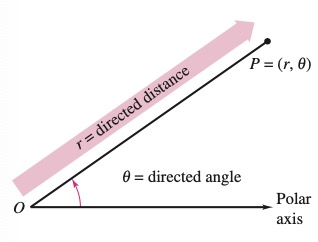
\includegraphics[width=0.60\linewidth]{Example_80.jpg} 
\end{minipage}
\end{mytheorem}

\newpage
 
 
The following equivalences hold:

\begin{enumerate}
    \item A point \( (r, \theta) \) can also be represented as \( (r, \theta + 2n\pi) \), where \( n \in \mathbb{Z} \) (any integer). That is,
    \[
    (r, \theta) = (r, \theta + 2n\pi).
    \]

    \item A point \( (r, \theta) \) can also be represented as \( (-r, \theta + (2n+1)\pi) \), where \( n \in \mathbb{Z} \). That is,
    \[
    (r, \theta) = (-r, \theta + (2n+1)\pi).
    \]

    \item In general, the point \( (r, \theta) \) can be written as:
    \[
    (r, \theta) = (r, \theta + 2n\pi) \quad \text{or} \quad (r, \theta) = (-r, \theta + (2n+1)\pi).
    \]
\end{enumerate}


\begin{tcolorbox}[colback=examplebg, colframe=red!75!black, title=\textbf{EXAMPLE 1: Equivalent Polar Coordinates}, fonttitle=\bfseries, sharp corners]
In the polar coordinate system, the point \( (3, \frac{\pi}{6}) \) has multiple representations. Write two equivalent polar coordinate representations of this point.


\tcblower
\textbf{Solution:} 
In polar coordinates, a point \( (r, \theta) \) can be represented as:
\begin{enumerate}
    \item \( (r, \theta + 2n\pi) \), where \( n \) is any integer.
    \item \( (-r, \theta + (2n+1)\pi) \), where \( n \) is any integer.
\end{enumerate}

\textbf{First Representation:} \\
Using the formula \( (r, \theta + 2n\pi) \):
\[
(3, \frac{\pi}{6} + 2\pi) = (3, \frac{13\pi}{6}).
\]

\textbf{Second Representation:} \\
Using the formula \( (-r, \theta + (2n+1)\pi) \):
\[
(-3, \frac{\pi}{6} + \pi) = (-3, \frac{7\pi}{6}).
\]
\end{tcolorbox}


\newpage
\subsubsection{Coordinate Conversion}
\begin{mytheorem}{Coordinate Conversion}{}

\begin{enumerate}
    \item \textbf{Polar-to-Rectangular:}
    \[
    x = r \cos \theta, \quad y = r \sin \theta.
    \]

    \item \textbf{Rectangular-to-Polar:}
    \[
    r^2 = x^2 + y^2, \quad \tan \theta = \frac{y}{x}.
    \]
\end{enumerate}

\begin{minipage}{\linewidth}
    \centering
    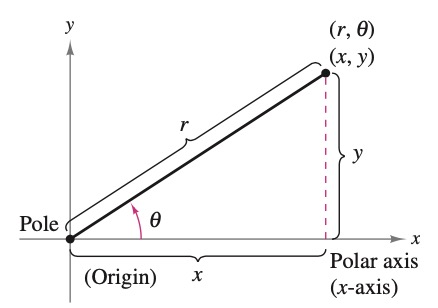
\includegraphics[width=0.45\linewidth]{Example_81.jpg} 
\end{minipage}
\end{mytheorem}


\begin{tcolorbox}[colback=examplebg, colframe=red!75!black, title=\textbf{EXAMPLE 1: Polar-to-Rectangular Conversion}, fonttitle=\bfseries, sharp corners]

Convert the following polar coordinates to rectangular coordinates:
\begin{enumerate}
    \item \( (r, \theta) = (2, \pi) \)
    \item \( (r, \theta) = \left(\sqrt{3}, \frac{\pi}{6}\right) \)
\end{enumerate}

\tcblower
\textbf{Solution:} 
\begin{enumerate}
    \item For \( (r, \theta) = (2, \pi) \):
    \[
    x = r \cos \theta = 2 \cos \pi = -2, \quad y = r \sin \theta = 2 \sin \pi = 0.
    \]
    Therefore, the rectangular coordinates are \( (x, y) = (-2, 0) \).

    \item For \( (r, \theta) = \left(\sqrt{3}, \frac{\pi}{6}\right) \):
    \[
    x = \sqrt{3} \cos \frac{\pi}{6} = \sqrt{3} \cdot \frac{\sqrt{3}}{2} = \frac{3}{2}, \quad
    y = \sqrt{3} \sin \frac{\pi}{6} = \sqrt{3} \cdot \frac{1}{2} = \frac{\sqrt{3}}{2}.
    \]
    Therefore, the rectangular coordinates are \( (x, y) = \left(\frac{3}{2}, \frac{\sqrt{3}}{2}\right) \).
\end{enumerate}
\end{tcolorbox}



\begin{tcolorbox}[colback=examplebg, colframe=red!75!black, title=\textbf{EXAMPLE 2: Rectangular-to-Polar Conversion}, fonttitle=\bfseries, sharp corners]

Convert the following rectangular coordinates to polar coordinates:
\begin{enumerate}
    \item \( (x, y) = (-1, 1) \)
\end{enumerate}

\tcblower
\textbf{Solution:} 
\begin{enumerate}
    \item For \( (x, y) = (-1, 1) \):
    \[
    \tan \theta = \frac{y}{x} = \frac{1}{-1} = -1 \implies \theta = \frac{3\pi}{4}.
    \]
    Since \( \theta \) was chosen to be in the same quadrant as \( (x, y) \), we calculate the magnitude:
    \[
    r = \sqrt{x^2 + y^2} = \sqrt{(-1)^2 + 1^2} = \sqrt{2}.
    \]
    Therefore, the polar coordinates are \( (r, \theta) = \left(\sqrt{2}, \frac{3\pi}{4}\right) \).
\end{enumerate}
\end{tcolorbox}

\begin{tcolorbox}[colback=examplebg, colframe=red!75!black, title=\textbf{EXAMPLE 3: Convert Polar Function to Cartesian Function}, fonttitle=\bfseries, sharp corners]
The polar equation is:
\[
r = 4 \sin \theta
\]
Convert Polar Function to Cartesian Function


\tcblower
\textbf{Solution:} 
Using the relationships between polar and Cartesian coordinates:
\[
x = r \cos \theta, \quad y = r \sin \theta, \quad r^2 = x^2 + y^2
\]
we substitute \( r \sin \theta = y \). Therefore:
\[
r = 4 \sin \theta \implies r = 4 \frac{y}{r}.
\]

Multiplying through by \( r \) (assuming \( r \neq 0 \)):
\[
r^2 = 4y.
\]

Finally, substituting \( r^2 = x^2 + y^2 \):
\[
x^2 + y^2 = 4y.
\]

\subsection*{Cartesian Form:}
\[
x^2 + y^2 - 4y = 0.
\]
\end{tcolorbox}


\subsubsection{Derivatives of Polar Functions}

\begin{mytheorem}{Derivetives of Polar Function}{}
    When working with polar functions of the form \( r = f(\theta) \), we calculate derivatives as follows:

\begin{itemize}
    \item The derivative \( \frac{dr}{d\theta} \) represents the rate of change of the radial distance \( r \) with respect to the angle \( \theta \).
    \item To find \( \frac{dr}{d\theta} \), differentiate the polar function \( r = f(\theta) \) as you would any regular function.
    \item The derivative \( \frac{dr}{d\theta} \) helps determine points where \( r \) changes most rapidly or points farthest from the origin in the polar coordinate system.
\end{itemize}
\end{mytheorem}

\begin{tcolorbox}[colback=examplebg, colframe=red!75!black, title=\textbf{EXAMPLE 4: Derivative of a Polar Function}, fonttitle=\bfseries, sharp corners]

Given the polar function \( r = 2 + \sin(\theta) \), find \( \frac{dr}{d\theta} \).

\tcblower
\textbf{Solution:} 

1. Start with the given polar function:
   \[
   r = 2 + \sin(\theta)
   \]

2. Differentiate \( r \) with respect to \( \theta \):
   \[
   \frac{dr}{d\theta} = \frac{d}{d\theta}[2 + \sin(\theta)]
   \]

3. Apply the derivative rules:
   \[
   \frac{dr}{d\theta} = 0 + \cos(\theta)
   \]

4. Thus, the derivative of the polar function is:
   \[
   \frac{dr}{d\theta} = \cos(\theta)
   \]
\end{tcolorbox}

\newpage
\subsubsection{Slope and Tangent Lines}

\begin{mytheorem}{Slope in Polar Form}{}

If \( f \) is a differentiable function of \( \theta \), then the \textit{slope} of the tangent line to the graph of \( r = f(\theta) \) at the point \( (r, \theta) \) is given by:
\[
\frac{dy}{dx} = \frac{\frac{dy}{d\theta}}{\frac{dx}{d\theta}} = 
\frac{f(\theta) \cos \theta + f'(\theta) \sin \theta}{-f(\theta) \sin \theta + f'(\theta) \cos \theta},
\]
provided that \( \frac{dx}{d\theta} \neq 0 \) at \( (r, \theta) \).

\end{mytheorem}
\begin{minipage}{\linewidth}
    \centering
    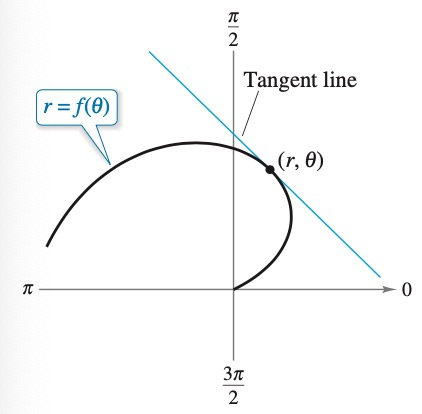
\includegraphics[width=0.40\linewidth]{Example_82.jpg} 
\end{minipage}

\begin{Note}{Conditions for Tangents in Polar Coordinates}{}
    \begin{enumerate}
    \item Solutions of \( \frac{dy}{d\theta} = 0 \) yield \textbf{horizontal tangents}, provided that \( \frac{dx}{d\theta} \neq 0 \).
    \item Solutions of \( \frac{dx}{d\theta} = 0 \) yield \textbf{vertical tangents}, provided that \( \frac{dy}{d\theta} \neq 0 \).
\end{enumerate}

If \( \frac{dy}{d\theta} \) and \( \frac{dx}{d\theta} \) are \textit{simultaneously} \( 0 \), then no conclusion can be drawn about tangent lines.
\end{Note}

\begin{tcolorbox}[colback=examplebg, colframe=red!75!black, title=\textbf{EXAMPLE 5: Find the EOTL}, fonttitle=\bfseries, sharp corners]

Find the equation of the line tangent to the polar curve \( r = \theta + \cos(2\theta) \) at \( \theta = \frac{\pi}{3} \).

\tcblower
\textbf{Solution:} 
We begin by calculating \( \frac{dy}{dx} \) using the polar derivatives:
\[
\frac{dy}{dx} = \frac{\frac{dy}{d\theta}}{\frac{dx}{d\theta}}
\]

The expressions for \( x \) and \( y \) in terms of \( r \) and \( \theta \) are:
\[
x = r \cos\theta, \quad y = r \sin\theta.
\]

Using the product rule for derivatives:
\[
\frac{dy}{d\theta} = \frac{d}{d\theta}\big(\theta \sin\theta + \sin\theta \cos(2\theta)\big)
\]
\[
= \sin\theta + \theta \cos\theta + \cos\theta \cos(2\theta) - 2\sin\theta \sin(2\theta),
\]

and
\[
\frac{dx}{d\theta} = \frac{d}{d\theta}\big(\theta \cos\theta + \cos\theta \cos(2\theta)\big)
\]
\[
= \cos\theta - \theta \sin\theta - \sin\theta \cos(2\theta) + 2\cos\theta \sin(2\theta).
\]

Substitute \( \theta = \frac{\pi}{3} \):
\[
\frac{dy}{dx} = \frac{\sin\frac{\pi}{3} + \frac{\pi}{3}\cos\frac{\pi}{3} + \cos\frac{\pi}{3}\cos\frac{2\pi}{3} - 2\sin\frac{\pi}{3}\sin\frac{2\pi}{3}}{\cos\frac{\pi}{3} - \frac{\pi}{3}\sin\frac{\pi}{3} - \sin\frac{\pi}{3}\cos\frac{2\pi}{3} + 2\cos\frac{\pi}{3}\sin\frac{2\pi}{3}}.
\]

This simplifies to:
\[
\frac{dy}{dx} = 0.429.
\]

Next, calculate the Cartesian coordinates of the tangent line:
\[
x = r \cos\theta = \left(\frac{\pi}{3} + \cos\frac{2\pi}{3}\right)\cos\frac{\pi}{3},
\]
\[
x = 0.274.
\]

\[
y = r \sin\theta = \left(\frac{\pi}{3} + \cos\frac{2\pi}{3}\right)\sin\frac{\pi}{3},
\]
\[
y = 0.474.
\]

Thus the equation of the tangent line is
\[y-0.474 = 0.429(x-0.274）\]

\end{tcolorbox}

\begin{tcolorbox}[colback=examplebg, colframe=red!75!black, title=\textbf{EXAMPLE 6: Finding Horizontal and Vertical Tangent Lines}, fonttitle=\bfseries, sharp corners]

Find the horizontal and vertical tangent lines of the polar curve \( r = \sin \theta \), for \( 0 \leq \theta \leq \pi \).

\tcblower
\textbf{Solution:} 
\begin{enumerate}
    \item Begin by expressing the curve in parametric form:
    \[
    x = r \cos \theta = \sin \theta \cos \theta,
    \]
    \[
    y = r \sin \theta = \sin \theta \sin \theta = \sin^2 \theta.
    \]

    \item Differentiate \( x \) and \( y \) with respect to \( \theta \):
    \[
    \frac{dx}{d\theta} = \cos^2 \theta - \sin^2 \theta = \cos 2\theta,
    \]
    \[
    \frac{dy}{d\theta} = 2 \sin \theta \cos \theta = \sin 2\theta.
    \]

    \item Solve for horizontal tangent lines by setting \( \frac{dy}{d\theta} = 0 \):
    \[
    \sin 2\theta = 0 \implies \theta = 0, \frac{\pi}{2}.
    \]

    \item Solve for vertical tangent lines by setting \( \frac{dx}{d\theta} = 0 \):
    \[
    \cos 2\theta = 0 \implies \theta = \frac{\pi}{4}, \frac{3\pi}{4}.
    \]

    \item Calculate the points of tangency:
    \begin{itemize}
        \item Horizontal tangent lines:
        \[
        \theta = 0 \implies r = \sin 0 = 0 \implies (x, y) = (0, 0),
        \]
        \[
        \theta = \frac{\pi}{2} \implies r = \sin \frac{\pi}{2} = 1 \implies (x, y) = (1, \frac{\pi}{2}).
        \]

        \item Vertical tangent lines:
        \[
        \theta = \frac{\pi}{4} \implies r = \sin \frac{\pi}{4} = \frac{\sqrt{2}}{2} \implies (x, y) = \left(\frac{\sqrt{2}}{2}, \frac{\pi}{4}\right),
        \]
        \[
        \theta = \frac{3\pi}{4} \implies r = \sin \frac{3\pi}{4} = \frac{\sqrt{2}}{2} \implies (x, y) = \left(\frac{\sqrt{2}}{2}, \frac{3\pi}{4}\right).
        \]
    \end{itemize}
\end{enumerate}
\end{tcolorbox}


\newpage 
\subsection{Area Bounded
by a Single Polar Curve}

\begin{mytheorem}{Area in Polar Coordinates}{}

If \( f \) is continuous and nonnegative on the interval \([ \alpha, \beta ]\), where \( 0 < \beta - \alpha \leq 2\pi \), then the area of the region bounded by the graph of \( r = f(\theta) \) between the radial lines \( \theta = \alpha \) and \( \theta = \beta \) is given by:
\[
A = \frac{1}{2} \int_\alpha^\beta \left[ f(\theta) \right]^2 \, d\theta
\]
or equivalently:
\[
A = \frac{1}{2} \int_\alpha^\beta r^2 \, d\theta,
\]
where \( 0 < \beta - \alpha \leq 2\pi \).

\begin{minipage}{\linewidth}
    \centering
    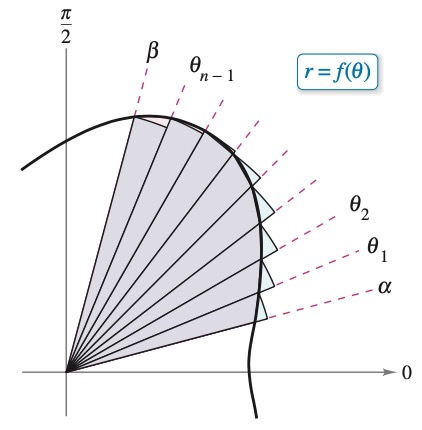
\includegraphics[width=0.40\linewidth]{Example_83.jpg} 
\end{minipage}
    
\end{mytheorem}

\begin{tcolorbox}[colback=examplebg, colframe=red!75!black, title=\textbf{EXAMPLE 1: Area of One Petal of a Rose Curve}, fonttitle=\bfseries, sharp corners]
Find the area of one petal of the rose curve \( r = 3 \cos 3\theta \).
\begin{minipage}{\linewidth}
    \centering
    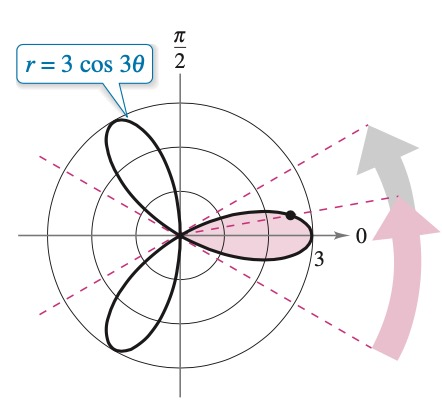
\includegraphics[width=0.35\linewidth]{Example_84.jpg} 
\end{minipage}


\tcblower
\textbf{Solution:} 


Using the formula for the area in polar coordinates:
\[
A = \frac{1}{2} \int_{\alpha}^{\beta} r^2 \, d\theta
\]
we calculate the area of one petal, where the petal is traced as \(\theta\) increases from \(-\pi/6\) to \(\pi/6\). Substituting \(r = 3 \cos 3\theta\):
\[
A = \frac{1}{2} \int_{-\pi/6}^{\pi/6} (3 \cos 3\theta)^2 \, d\theta.
\]

Simplify:
\[
A = \frac{1}{2} \int_{-\pi/6}^{\pi/6} 9 \cos^2 3\theta \, d\theta = \frac{9}{2} \int_{-\pi/6}^{\pi/6} \cos^2 3\theta \, d\theta.
\]

Using the power-reducing formula \(\cos^2 x = \frac{1 + \cos 2x}{2}\):
\[
A = \frac{9}{2} \int_{-\pi/6}^{\pi/6} \frac{1 + \cos 6\theta}{2} \, d\theta = \frac{9}{4} \int_{-\pi/6}^{\pi/6} (1 + \cos 6\theta) \, d\theta.
\]

Split the integral:
\[
A = \frac{9}{4} \left[ \int_{-\pi/6}^{\pi/6} 1 \, d\theta + \int_{-\pi/6}^{\pi/6} \cos 6\theta \, d\theta \right].
\]

Evaluate each integral:
\[
\int_{-\pi/6}^{\pi/6} 1 \, d\theta = \left[ \theta \right]_{-\pi/6}^{\pi/6} = \pi/6 - (-\pi/6) = \pi/3,
\]
\[
\int_{-\pi/6}^{\pi/6} \cos 6\theta \, d\theta = \left[ \frac{\sin 6\theta}{6} \right]_{-\pi/6}^{\pi/6} = \frac{\sin(\pi)}{6} - \frac{\sin(-\pi)}{6} = 0.
\]

Thus:
\[
A = \frac{9}{4} \left( \frac{\pi}{3} + 0 \right) = \frac{9}{4} \cdot \frac{\pi}{3} = \frac{3\pi}{4}.
\]
\end{tcolorbox}

\begin{tcolorbox}[colback=examplebg, colframe=red!75!black, title=\textbf{EXAMPLE 2: Area of One Petal of a Rose Curve}, fonttitle=\bfseries, sharp corners]

Find the area inside the smaller loop of the limaçon given by:
\[
r = 2\sin\theta + 1.
\]


\tcblower
\textbf{Solution:} 

To determine the bounds of integration, we set \( r = 0 \):
\[
0 = 2\sin\theta + 1 \implies \sin\theta = -\frac{1}{2}.
\]

The solutions for \( \sin\theta = -\frac{1}{2} \) are:
\[
\theta = \frac{7\pi}{6}, \quad \theta = \frac{11\pi}{6}.
\]

Thus, the bounds for the inner loop are \( \theta \in \left[\frac{7\pi}{6}, \frac{11\pi}{6}\right] \).

The area of the inner loop is given by:
\[
A = \frac{1}{2} \int_{\frac{7\pi}{6}}^{\frac{11\pi}{6}} \left( 2\sin\theta + 1 \right)^2 \, d\theta = 0.54
\]






\end{tcolorbox}

\newpage
\subsection{Area of the Region Bounded by Two Polar Curves}

\begin{Note}{Area in Polar Coordinates}{}

If \( f \) is continuous and nonnegative on the interval \([ \alpha, \beta ]\), where \( 0 < \beta - \alpha \leq 2\pi \), then the area of the region bounded by the graph of \( r = f(\theta) \) between the radial lines \( \theta = \alpha \) and \( \theta = \beta \) is given by:
\[
A = \frac{1}{2} \int_\alpha^\beta \left[ f(\theta) \right]^2 \, d\theta
\]
or equivalently:
\[
A = \frac{1}{2} \int_\alpha^\beta r^2 \, d\theta,
\]
where \( 0 < \beta - \alpha \leq 2\pi \).

    
\end{Note}

\begin{Note}{Points of Intersection of Polar Graphs}{}
    

To find the points of intersection of two polar equations, solve the equations simultaneously. For example:

Given the equations:
\[
r = 1 - 2\cos\theta \quad \text{and} \quad r = 1,
\]

1. Substitute \( r = 1 \) from the second equation into the first:
   \[
   1 = 1 - 2\cos\theta.
   \]

2. Simplify:
   \[
   \cos\theta = 0.
   \]

3. Solve for \( \theta \):
   \[
   \theta = \frac{\pi}{2}, \quad \theta = \frac{3\pi}{2}.
   \]

Thus, the points of intersection occur at:
\[
r = 1, \quad \theta = \frac{\pi}{2} \quad \text{and} \quad \theta = \frac{3\pi}{2}.
\]



\begin{minipage}{\linewidth}
    \centering
    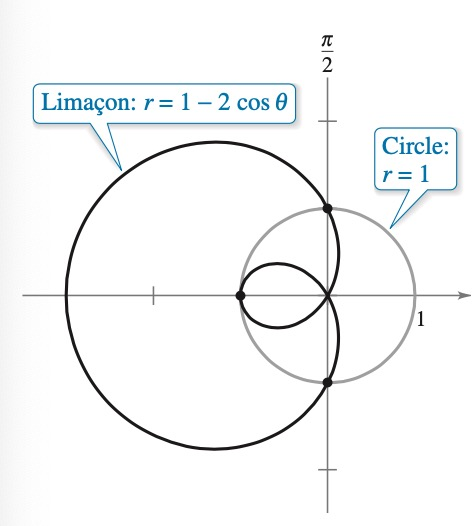
\includegraphics[width=0.30\linewidth]{Example_85.jpg} 
\end{minipage}
\end{Note}

\begin{tcolorbox}[colback=examplebg, colframe=red!75!black, title=\textbf{EXAMPLE 1: Find the Integral of the Function}, fonttitle=\bfseries, sharp corners]

Find the area of the region common to the two curves:
\[
r = -6\cos\theta \quad \text{(Circle)}
\]
and
\[
r = 2 - 2\cos\theta \quad \text{(Cardioid)}.
\]

\tcblower
\textbf{Solution:} 
The region common to the two curves is divided into two parts:
\begin{itemize}
    \item From $\theta = \frac{\pi}{2}$ to $\theta = \frac{2\pi}{3}$: the region between the circle and the radial line.
    \item From $\theta = \frac{2\pi}{3}$ to $\theta = \pi$: the region between the cardioid and the radial line.
\end{itemize}

The total area is given by:
\[
A = 2 \left( \int_{\pi/2}^{2\pi/3} \frac{1}{2}(-6\cos\theta)^2 \, d\theta + \int_{2\pi/3}^{\pi} \frac{1}{2}(2 - 2\cos\theta)^2 \, d\theta \right).
\]

Simplify each integral:
\[
\int_{\pi/2}^{2\pi/3} \frac{1}{2}(-6\cos\theta)^2 \, d\theta = \int_{\pi/2}^{2\pi/3} 18\cos^2\theta \, d\theta,
\]
and use the power-reduction formula $\cos^2\theta = \frac{1 + \cos(2\theta)}{2}$.

Similarly:
\[
\int_{2\pi/3}^{\pi} \frac{1}{2}(2 - 2\cos\theta)^2 \, d\theta = \int_{2\pi/3}^{\pi} \frac{1}{2}(4 - 8\cos\theta + 4\cos^2\theta) \, d\theta.
\]

Evaluate both integrals and sum them to obtain:
\[
A = \frac{5\pi}{2}.
\]

Thus, the total area is:
\[
\text{Area} = 5\pi \approx 15.7.
\]

\end{tcolorbox}



\
\end{document}
